\documentclass{beamer}
\usepackage{textcomp}
\usepackage{multimedia}
\usepackage{media9}

\usetheme{Rochester}
\usecolortheme{crane}

\definecolor{umber}{HTML}{A3C9F4}
\definecolor{light}{HTML}{DBECFF}

\setbeamercolor{frametitle}{fg=black, bg=umber}

\setbeamercolor{block body example}{bg=light}
\setbeamercolor{block title example}{bg=umber}


\setbeamercolor{frametitle}{fg=black}
\setbeamercolor{title}{fg=black, bg=umber}

\begin{document}

  \title[Crisis] % (optional, only for long titles)
  {Migration and Segregation in Three Dimensional Cellular Co-cultures}
  \subtitle{Role of Differential Cell Adhesion and Elasticity}
  \author[Author, Kolbman] % (optional, for multiple authors)
  {Dan Kolbman\\Mentor: Moumita Das}
  \date[2014]
  {Capstone I, Winter 2014}
  \subject{info}

  \frame{\titlepage}


  \begin{frame}
    \frametitle{Background}
    \framesubtitle{Behavior of cancer cells}
    \includemovie{.85\textheight}{.85\textheight}{cancercancer.mp4}

    \includemedia[
      label=vidA,
      addresource=cancercancer.mp4,
      activate=pageopen,
      width=5cm, height=4cm,
      flashvars={
         source=cancercancer.mp4
        &loop=true
      }
    ]{}{VPlayer.swf}

    \vfill
    
  \end{frame}  
  
  % BACKGROUND %
  % Provide background about the subject. Talk about the different physical propreties %
  % and how they're thought to affect cancer migration and segregation %
  \begin{frame}
    \frametitle{Background}
    \framesubtitle{Behavior of cancer cells}
    
    \begin{itemize}
    \item Cancer cells are mechanically softer than healthy cells of the same tissue type. 
    (Lee et al. Biophysical Journal 2012).
    \item Cancer cells show much less cell-cell adhesion than non-cancerous cells  due to deficiency of the protein E-cadherin. 
    (Cukierman et al., Science 2001)
    \item Cancer cells move more quickly in populations of healthy cells in 2D co-cultures. 
    (Lee et al, Biophysical Journal 2012, Butcher et al. unpublished).
    \end{itemize}
    \vfill
    
  \end{frame}  
  

  % MODEL %
  % Discuss the general langevin equation for the dynamics of the system %
  \begin{frame}
    \frametitle{The Model}
    Minimum Ingredients
    \begin{itemize}
    \item Binary system of colloids 
    \item Activity (self-driven forces due to ATP consumption)
    \item Cell deformability
    \item Cell-cell adhesion
    \item Confinement
    \end{itemize}
    
	\begin{exampleblock}{Over Damped Langevin Equation}
	$$\vec{F}(\vec{r _m}) - \gamma \frac{d\vec{r_m}}{dt} + \vec{\eta}(t) = 0$$
	\end{exampleblock}
	\begin{columns}[t]
    \column{.5\textwidth}
     $\vec{F}$ -- Total force on the cell \\
     $\gamma$ -- The damping coefficient \\
      $\vec{r_m}$ -- Particle position. \\
    \column{.5\textwidth}
    $\vec{\eta}$ -- Fluctuating force to approximate collisions with smaller particles \\
    \end{columns}
    
    \vfill
    
  \end{frame}

  % INTERACTION FORCES %
  \begin{frame}
    \frametitle{2D Model}
    \framesubtitle{Interaction Forces}
    % Initial system state %
    \begin{figure}
      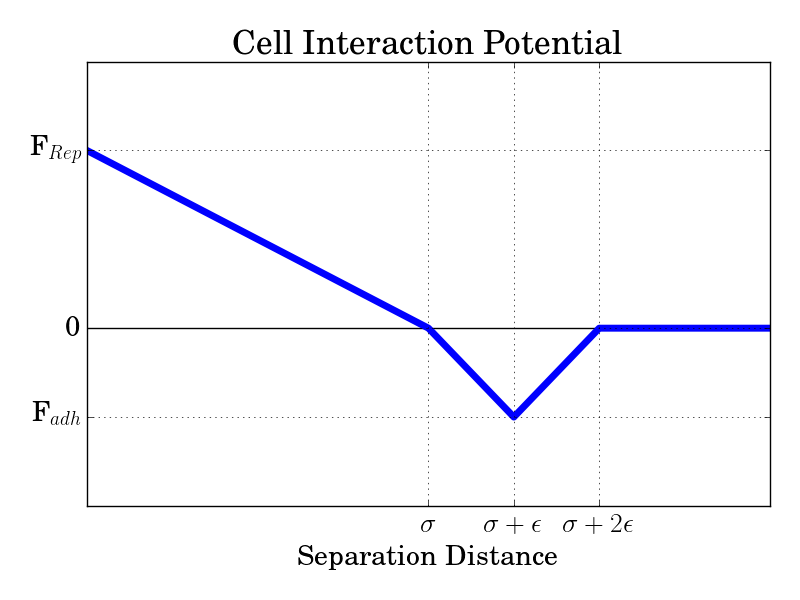
\includegraphics[width=3in]{interaction.png}
      \caption{Interaction Potential}
    \end{figure}

    \vfill
  \end{frame}
  
  %%%% RESULTS FOR 2D %%%%
  % THE SIMULATION SYSTEM %
  \begin{frame}
    \frametitle{2D Model}
    \framesubtitle{Force Contributions}
    % Final system state %
    \begin{figure}
      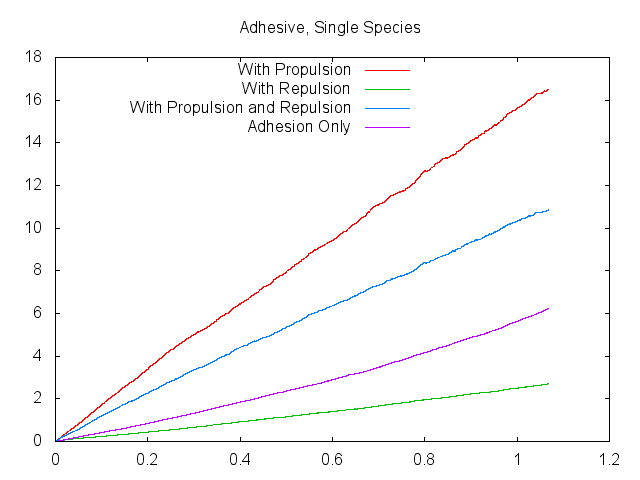
\includegraphics[width=3.3in]{msd2D.png}
      \caption{Single species system with different forces active}
    \end{figure}
    \vfill
  \end{frame}

  % ADHESION %
  \begin{frame}
    \frametitle{2D Model}
    \framesubtitle{Effect of adhesion}
    \begin{figure}
      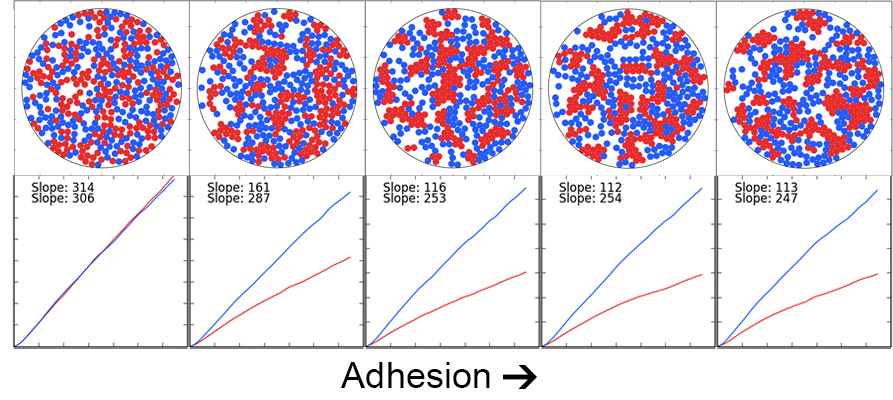
\includegraphics[width=4.5in]{adhinc.jpg}
      \caption{Red - Healthy Cells, Blue - Cancerous Cells}
    \end{figure}
    \vfill
  \end{frame}


  % PHASE DIAGRAM %
  \begin{frame}
    \frametitle{2D Model}
    \framesubtitle{Phase Diagram}
    \begin{columns}[t] 
    \column{0.5\textwidth}
    \begin{figure}
    \end{figure}
    \column{0.5\textwidth}
    \begin{figure}
    \end{figure}
    \end{columns}
    \vfill
  \end{frame}
  

  % MOTIVATION %
  % Motivate the need for a 3d version of the model %
  \begin{frame}
    \frametitle{Motivation for a 3D Model}
    \framesubtitle{New experimental data}
    
    \begin{itemize}
    \item Cells move at different rates in $2D$ than in $3D$.
    (Cukierman et al., Science 2001)
    \item Cells move differently when confined in an extracellular matrix (ECM). 
    (Doyle et al., J. Cell Biol. 2009)       
    \item New experiments and techniques are becoming available to observe cellular co-cultures in $3D$
    
    \item Little theoretical understanding of biomechanics and biophysics of cell co-cultures existing in $3D$
    \end{itemize}
    
    
	\center\emph{Can we propose a new model of cancer cell aggregation and migration in $3D$? \\
	Can we obtain insights from these results about the underlying physical mechanism of metastasis?}
    
    \vfill
    
  \end{frame}
    
  % EXPERIMENTAL %
  \begin{frame}
    \frametitle{Experimental Results}
    \framesubtitle{MSD}
    \begin{figure}
    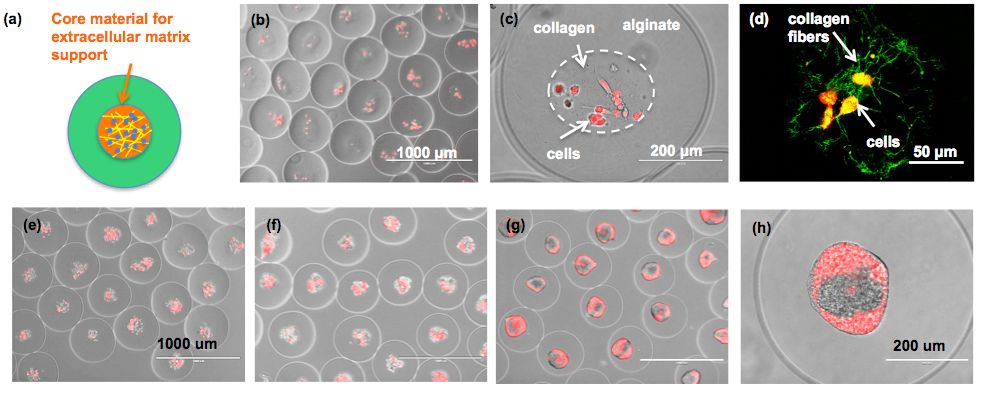
\includegraphics[width=3.4in]{MMaMWufig.png}
    \caption{Core-shell hydrogel microcapsules with ECM support for 3D confined cell culture. (a) A schematic of an ECM-supported microcapsule. (b) MDA-MB-231 cells with tomato red expression encapsulated within collagen matrix. (c) A magnified view of a single microcapsule. (d) Cells in the collagen fibers (green) in the inner layer of a microcapsule (e-h) Cell segregation under 3D confinement: MDA-MB-231 (with red Tomato fluorescence) and MCF-10A cells.
Experimental collaboration: M. Wu and M. Ma, Cornell University}
    \end{figure}
    \vfill
  \end{frame}
    
  % EXPERIMENTAL %
  \begin{frame}
    \frametitle{Experimental Conditions}
  	\begin{columns}[t] 
  	\column{0.5\textwidth}
  	\begin{figure}
  	  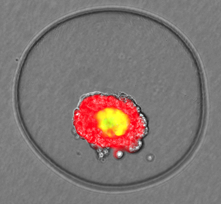
\includegraphics[height=1.0in]{minglin.png}
  	  \caption{An expiremental microcapsule with a cellular co-culture.
Collaboration: M. Ma, M. Wu, Cornell University}
  	\end{figure}
    \column{.5\textwidth}
    \begin{figure}
      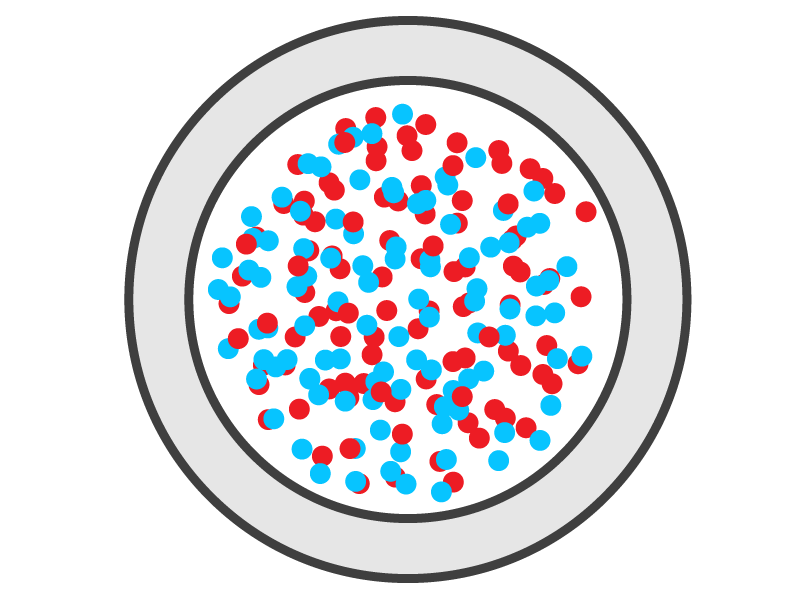
\includegraphics[height=1.0in]{Fig1.png}
      \caption{An ideal microcapsule containing a cellular co-culture}
    \end{figure}
    \end{columns}
    \begin{centering}
    Inner diameter -- $50-700$ \textmu m\\
    Outer diameter -- $400-7000$ \textmu m\\
	  Cell diameter -- $\sim 10$ \textmu m\\
    \end{centering}
    \vfill
  \end{frame}

  % 3D conf, msd %
  \begin{frame}
    \frametitle{3D Model}
    \framesubtitle{}
  	\begin{columns}[t] 
  	\column{0.5\textwidth}
  	\begin{figure}
  	  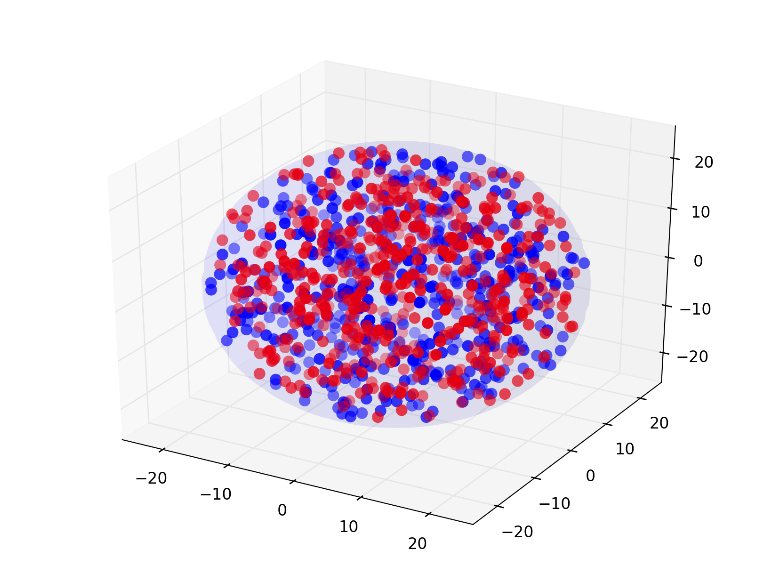
\includegraphics[height=1.6in]{3dconf.png}
      \caption{Configuration for 3D Co-culture.}
  	\end{figure}
    \column{.5\textwidth}
    \begin{figure}
      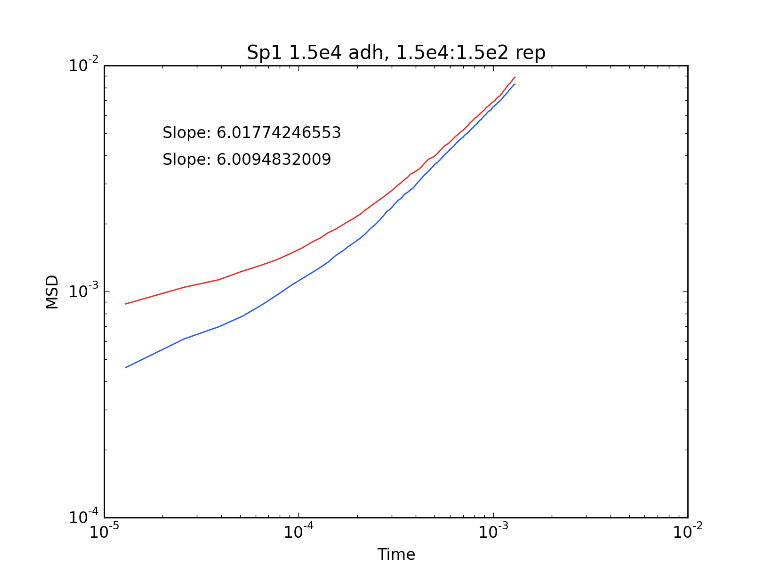
\includegraphics[height=1.6in]{3dmsd.png}
      \caption{MSD for 3D Co-culture.}
    \end{figure}
    \end{columns}
    \vfill
  \end{frame}
  
  % FUTURE GOALS %
  \begin{frame}
    \frametitle{Future Goals}
    \framesubtitle{}
    \begin{itemize}
    \item Add ECM in the form of a disordered potential
    \item Account for mitosis
    \item Run for longer time scales
    \end{itemize}
    \vfill
  \end{frame}
  
    
\end{document}
